\chapter{Programming using Bootloader}

\emph{Bootloader} is a short program used to burn the firmware to the microcontroller without any programmer device. It is the first thing to run on device power on and is accessible through the serial interface.

\section{USB connection (obsolete)}

Setup described in this section enables you to program Main Boards using wired connection (i.e. mini USB cable) Bootloader.

\subsection{Programming the Bootloader on Main Board}
\label{subsec:programming_the_bootloader}

A prerequisite to using Bootloader to program the Main Board is having the Bootloader itself configured and programmed onto the board. USB (wired) Bootloader is provided in \texttt{UART\_BOOTLOADER} project of PSoC creator \texttt{MU31S-000} workspace.

Steps:
\begin{enumerate}
	\item Build the project (right click on project name > Build \texttt{UART\_BOOTLOADER}).
	\item Set \texttt{UART\_BOOTLOADER} project to active (right click on project name > Set As Active Project).
	\item Connect MiniProg to MB and the PC.
	\item Program the MB (\textit{program} button in PSoC creator or Ctrl+F5).
	\item If asked, select a device to program. Sometimes the connection between MB and MiniProg is bad so make sure you adjust the cable until the device \texttt{PSoC 5LP CY8C5888LTI*-LP097} is detected. %TODO version??
	\item Once the device is detected, select \texttt{Port Acquire} > \texttt{Connect} > \texttt{OK} and wait for the completion of programming process.
\end{enumerate}

\subsection{Programming MB using Bootloader}
\label{subsec:programming_with_bootloader}

In order to program Main Board using Bootloader, \texttt{Bootloadable} component on MB has to be running and awaiting for programming request. It can be achieved by setting a waiting time after each system power on during which MB enters this mode. It is, however, not efficient because we sometimes need to program MB without power cycling it. Therefore, programs devised for Main Board always need to have one \textit{interpreter} task running which activates Bootloadable on request. This mode is entered by sending \texttt{'b'} character to MB's general purpose (debugging) UART.

\begin{figure}[htb]
    \centering
	  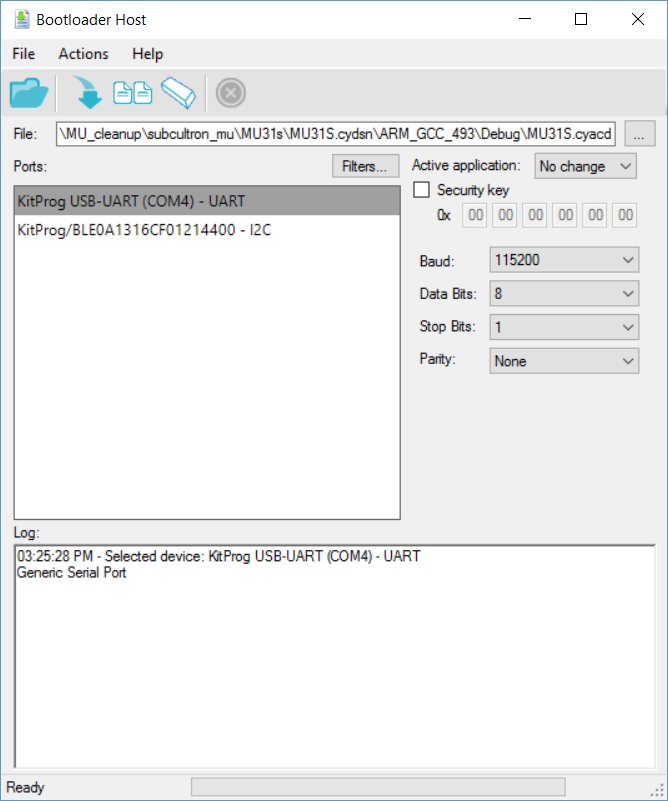
\includegraphics[width=0.6\linewidth]{figures/Bootloader_BLE.png}
	\caption{Setting up Bootloader Host}
	\label{fig:bootloader_host}
\end{figure}

The next step is to connect to the Main Board and start the programming process.\\
Steps:
\begin{enumerate}
	\item Connect the MB to your PC via mini USB cable. Make sure all connections to this COM port are closed (stop connections in Docklight).
	\item Open the project you wish to program in PSoC Creator.
	\item Go to \texttt{Tools} > \texttt{Bootloader Host}.
	\item Select the correct COM port and adjust settings to match the ones in Figure \ref{fig:bootloader_host}.
	\item Click on \texttt{Program} button and wait for the process to execute.
\end{enumerate}

\section{BLE Bootloader (obsolete)}

The process of programming MB using BLE Bootloader is the same as the one using wired connection Bootloader.
The only difference is in the way the connection to the device is established (step 1 in the previous section).
For guide on setting up BLE bridge between MB and PC, refer to Chapter \ref{ch:connecting_to_ble}.
Bootloader project that needs to be programmed onto the Main Board is \texttt{UART\_Bootloader\_BLE}.

\section{I2C Bootloader}

The process of programming MB using I2C Bootloader differs from previous described ones.
The process of programming I2C Bootloader stays the same, only the name of the project changes to \texttt{I2C\_Bootloader.cydsn} in Main Board case, or in eSense board case \texttt{I2C\_Bootloader\_eSense.cydsn}.
Desired program is transferred to aMussel's Raspberry Pi over WiFi.
Programming is done over I2C, where Raspberry Pi reprograms the Main Board.
Detailed description is described in \ref{subsec:win_prog_app}.


Next step is the programming process.\\
Steps:
\begin{enumerate}
	\item Build the project you wish to program in PSoC Creator.
	\item Put Main Board in Bootloader mode.
	%TODO over what interface
	\item Make sure Access Point router is turned on (and setup properly).
	\item Wait for aMussel to boot up the Raspberry Pi 
	%TODO modify bootloader to change colors depending on the state
	\item Open aMussel programming GUI and follow programming steps described in \ref{subsec:win_prog_app}.
	\item Wait for programming to finish.
\end{enumerate}

\subsection{Windows programming application}
\label{subsec:win_prog_app}

\begin{figure} [h!]
%\hfill
\subfloat[Main screen]{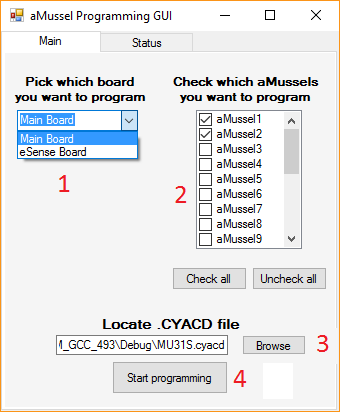
\includegraphics[width=3.8cm]{./figures/programming_gui_main_screen_boards.png}}
\label{subflo:windows_programming_application_main}
\hfill
\subfloat[Status screen - Idle]{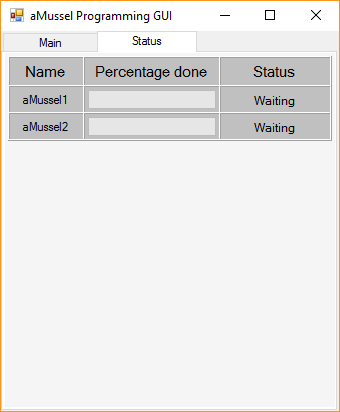
\includegraphics[width=3.8cm]{./figures/programming_gui_status_screen.png}}
\hfill
\subfloat[Status screen - Transfering code]{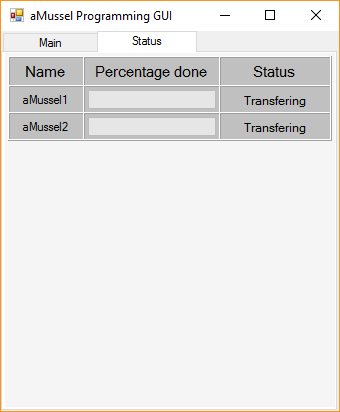
\includegraphics[width=3.8cm]{./figures/programming_gui_status_screen_transfering.png}}
%\hfill
\vfill
%\hfill
\subfloat[Status screen - Compiling code]{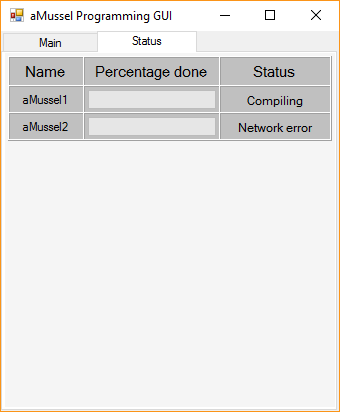
\includegraphics[width=3.8cm]{./figures/programming_gui_status_screen_compiling.png}}
\hfill
\subfloat[Status screen - Programming code]{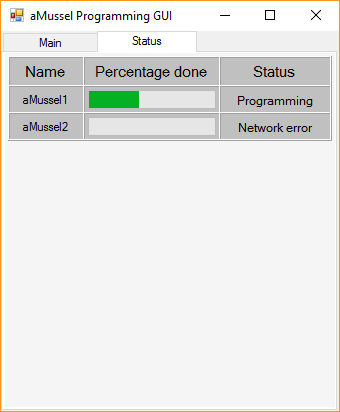
\includegraphics[width=3.8cm]{./figures/programming_gui_status_screen_programming.png}}
\hfill
\subfloat[Status screen - Programming done]{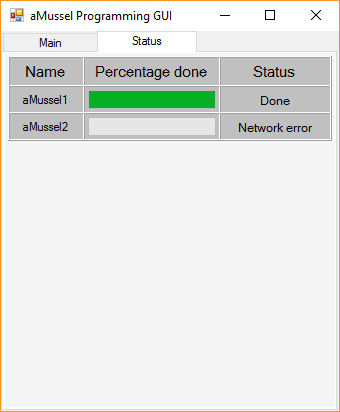
\includegraphics[width=3.8cm]{./figures/programming_gui_status_screen_done.png}}
%\hfill
\caption{Windows programming application}
\label{fig:windows_programming_application}
\end{figure}
%TODO change figures to the latest version

To make the process of reprogramming robotic swarm easy, an automated programming application was made.
The application was made in Visual Studio, using the Visual C++ programming language.

The programming procedure is divided in five steps:
\begin{itemize}
\item Choosing a programming configuration
\item Starting the programming procedure
\item Transferring the binary file containing the code
\item Compiling the program on RaspberryPI for programming the PSoC board over I2C
\item Executing the compiled program

\end{itemize}

As shown in \ref{fig:windows_programming_application}a), choosing a programming configuration is split in three steps:
\begin{itemize}
\item Choosing the appropriate board
\item Choosing which aMussels the operator wants to program
\item Choosing the binary file containing the code
\end{itemize}

Before the pressing \textit{Start programming} button in step 2., in the status tab aMussels 1 and 2 are shown to be in waiting mode (\ref{fig:windows_programming_application}b)).
After the programming procedure has started, the status indicator of each aMussel is indicating that the transferring procedure has started (\ref{fig:windows_programming_application}c)).
In case of an unsuccessful file transfer, the status indicator shows "Network error", as seen in aMussel2's status(\ref{fig:windows_programming_application}d)).
The compiling step is shown in \ref{fig:windows_programming_application}d in aMussel1's status.
In the final stage of the programming procedure, the progress bar indicates the percentage of flash memory currently transferred to the PSoC board (\ref{fig:windows_programming_application}e)).
After successful programming, the status indicator of aMussel1 is in the "Done" state and the aMussel should start executing the newly programmed code.

